% Four-slide English summary for the DeepSeek-CoT SFT experiment.
% Compiler: pdflatex

\documentclass[aspectratio=169,10pt]{beamer}

\usetheme{default}
\setbeamertemplate{navigation symbols}{}
\setbeamertemplate{footline}[frame number]
\setbeamertemplate{blocks}[default]

\usepackage{amsfonts,amsmath}
\usepackage{tabularx}
\usepackage{booktabs}
\usepackage{graphicx}
\usepackage{xcolor}
\usepackage[T1]{fontenc}
\usepackage{lmodern}
\usepackage{array}

\graphicspath{{images/}}

\definecolor{mainblue}{RGB}{28,78,122}
\definecolor{accentred}{RGB}{178,54,48}
\definecolor{accentgreen}{RGB}{27,120,55}
\setbeamercolor{frametitle}{fg=black,bg=white}
\setbeamerfont{frametitle}{series=\bfseries,size=\large}
\setbeamercolor{title}{fg=black}
\setbeamercolor{structure}{fg=mainblue}
\setbeamercolor{block title}{fg=black,bg=gray!12}
\setbeamercolor{block body}{fg=black,bg=white}

\newcommand{\good}[1]{\textcolor{mainblue}{\textbf{#1}}}
\newcommand{\warn}[1]{\textcolor{accentred}{\textbf{#1}}}
\newcommand{\markgreen}[1]{\textcolor{accentgreen}{\textbf{#1}}}
\newcommand{\smallgray}[1]{\textcolor{black!65}{\scriptsize #1}}

\title{DeepSeek-CoT SFT for Parametric Faithfulness}
\subtitle{LLaMA-3B + OpenBookQA + FUR}
\author{One-shot SFT extension}
\date{}

\begin{document}

\begin{frame}{Goal: Test Whether Distilled CoT Improves Faithfulness}
\small
\begin{columns}[T,onlytextwidth]
  \begin{column}{0.50\textwidth}
    \textbf{Research question}

    \vspace{0.35em}
    Can one SFT pass on \good{DeepSeek-revised CoTs} make a 3B model's
    generated reasoning more aligned with the parametric knowledge supporting
    its answers?

    \vspace{0.8em}
    \textbf{Base idea}
    \begin{itemize}
      \item Student: LLaMA-3.2-3B-Instruct.
      \item Teacher revises student CoTs, not just final answers.
      \item Evaluate with \good{Faithfulness by Unlearning Reasoning Steps} (FUR).
    \end{itemize}
  \end{column}

  \begin{column}{0.46\textwidth}
    \textbf{Pipeline}

    \vspace{0.35em}
    \begin{block}{1. Draft}
      Base LLaMA-3B generates OpenBookQA rationales.
    \end{block}
    \begin{block}{2. Revise}
      \texttt{deepseek-v4-pro} rewrites concise, answer-consistent CoTs.
    \end{block}
    \begin{block}{3. SFT + FUR}
      Fine-tune once, then compare Base vs. SFT on the same FUR test set.
    \end{block}
  \end{column}
\end{columns}

\vspace{0.5em}
\smallgray{FUR follows the paper ``Measuring Chain of Thought Faithfulness by Unlearning Reasoning Steps'' (arXiv:2502.14829).}
\end{frame}

\begin{frame}{Experimental Setup}
\small
\begin{columns}[T,onlytextwidth]
  \begin{column}{0.52\textwidth}
    \textbf{Data and SFT}

    \vspace{0.35em}
    \begin{tabularx}{\linewidth}{p{0.38\linewidth}>{\raggedright\arraybackslash}X}
      \toprule
      Base model & Llama-3.2-3B \\
      Teacher & \texttt{deepseek-v4-pro} \\
      Draft set & 2000 OpenBookQA train examples \\
      Accepted SFT data & 1852 examples (92.6\%) \\
      SFT method & LoRA, \texttt{down\_proj} only \\
      LoRA config & rank 32, alpha 64, dropout 0.05 \\
      Training & lr \(=10^{-4}\), 1 epoch, max len 512 \\
      \bottomrule
    \end{tabularx}
  \end{column}

  \begin{column}{0.44\textwidth}
    \textbf{FUR evaluation}

    \vspace{0.35em}
    \begin{tabularx}{\linewidth}{p{0.43\linewidth}>{\raggedright\arraybackslash}X}
      \toprule
      Target split & 100 OpenBookQA test questions \\
      Retain split & 20 held-out questions \\
      Compared arms & Base vs. DeepSeek-Rev. SFT \\
      Unlearning & NPO + KL \\
      FUR LR / epochs & \(3\times10^{-5}\) / 5 \\
      Updated params & \texttt{down\_proj} only \\
      Seed & 1001 \\
      \bottomrule
    \end{tabularx}

    \vspace{0.8em}
    \textbf{Primary readout.}
    Report FF-HARD/FF-SOFT on agreement questions; use the strict paired
    subset for uncertainty checks.
  \end{column}
\end{columns}
\end{frame}

\begin{frame}{Main Results: Accuracy, Controls, and Faithfulness}
\scriptsize
\begin{columns}[T,onlytextwidth]
  \begin{column}{0.62\textwidth}
    \centering
    \begin{tabular}{lrrrrrr}
      \toprule
      Model & Dir. & CoT & Agree & Steps & Eff. & Spec. \\
      \midrule
      Base & 70.00 & 73.00 & 82.00 & 6.37 & 92.58 & 94.04 \\
      SFT & \good{73.00} & \good{77.00} & \good{85.00} & \good{3.12} & \good{97.62} & \good{98.79} \\
      \bottomrule
    \end{tabular}

    \vspace{0.7em}
    \begin{tabular}{lrrrr}
      \toprule
      Model & Agree N & FF-HARD & FF-SOFT & Valid steps \\
      \midrule
      Base & 82 & 70.73 & 54.09 & 495 \\
      SFT & 85 & 65.88 & \good{56.07} & 311 \\
      \bottomrule
    \end{tabular}
  \end{column}

  \begin{column}{0.34\textwidth}
    \textbf{What changed?}
    \begin{itemize}
      \setlength{\itemsep}{0.35em}
      \item CoTs become shorter: \good{6.37 to 3.12} steps.
      \item FUR becomes cleaner: higher efficacy and specificity.
      \item Faithfulness is \warn{not clearly improved}: FF-SOFT rises, but FF-HARD falls.
    \end{itemize}

    \vspace{0.2em}
    \textbf{Paired check.}
    On 75 common agreement questions:
    \begin{itemize}
      \setlength{\itemsep}{0.2em}
      \item FF-HARD: \(-4.00\) pp, CI \([-16.00, 8.00]\).
      \item FF-SOFT: \(+1.12\) pp, CI \([-7.95, 9.95]\).
    \end{itemize}
  \end{column}
\end{columns}
\end{frame}

\begin{frame}{Visual Summary}
\small
\begin{columns}[T,onlytextwidth]
  \begin{column}{0.50\textwidth}
    \centering
    \textbf{FUR control region}

    \vspace{0.25em}
    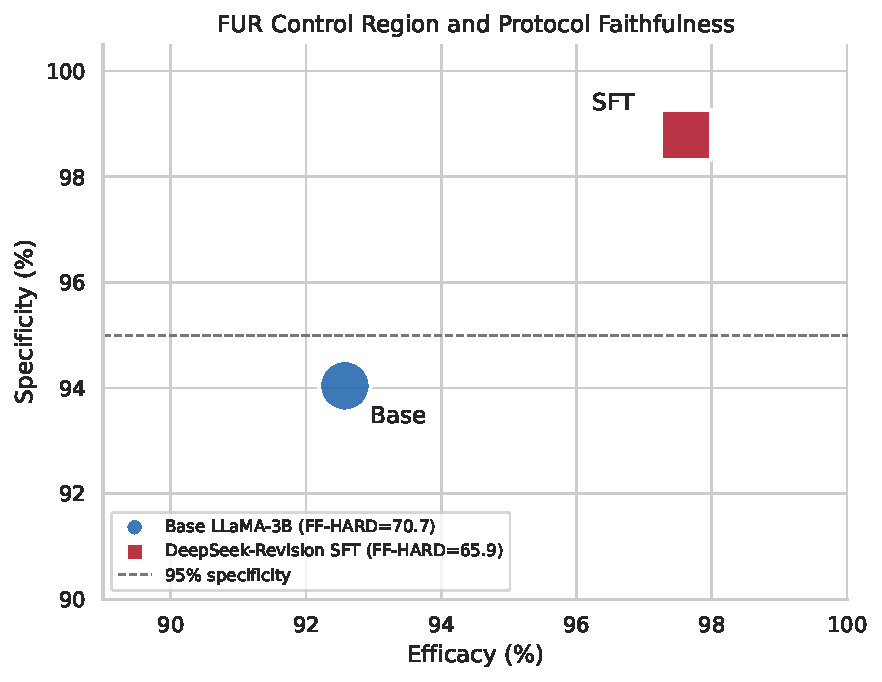
\includegraphics[width=\linewidth,height=0.62\textheight,keepaspectratio]{eff_spec_faithfulness.pdf}

    \vspace{0.2em}
    \scriptsize
    SFT moves to the high-efficacy, high-specificity region.
  \end{column}

  \begin{column}{0.50\textwidth}
    \centering
    \textbf{Protocol faithfulness}

    \vspace{0.25em}
    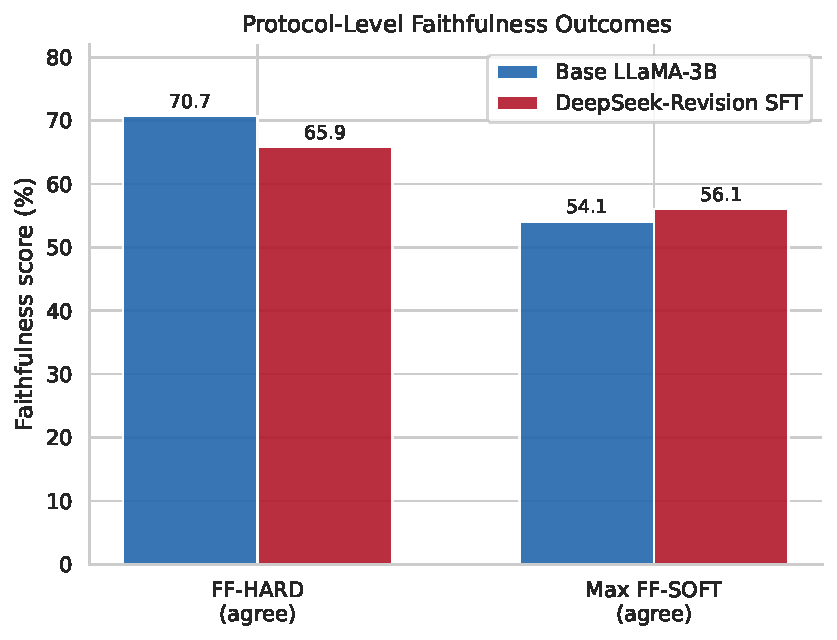
\includegraphics[width=\linewidth,height=0.62\textheight,keepaspectratio]{faithfulness_comparison.pdf}

    \vspace{0.2em}
    \scriptsize
    FF-SOFT improves slightly, while FF-HARD does not.
  \end{column}
\end{columns}

\vspace{0.55em}
\textbf{Takeaway.}
\good{One-shot distilled-CoT SFT improves compactness and FUR control quality.}
It does \warn{not yet establish a statistically stable faithfulness gain}.
\end{frame}

\end{document}
